\chapter{Background and Related Work}
\label{chap:background}

This chapter reviews the concepts and prior work on which this thesis builds.
Section~\ref{sec:bg-kg} introduces knowledge graphs and the graph data models
used to represent them, together with their use in the biomedical domain.
Section~\ref{sec:bg-ie} covers information extraction, the task of identifying
entities and relations in text, and the methods used to perform it.
Section~\ref{sec:bg-grounding} discusses hallucination in large language models
and techniques for grounding their output in an external source of knowledge.
Section~\ref{sec:bg-qg} reviews automatic question generation and the
educational frameworks used to describe question difficulty. Finally,
Section~\ref{sec:bg-guidelines} describes clinical practice guidelines and
efforts to represent them in a computable form, and
Section~\ref{sec:bg-related} discusses the work most closely related to this
thesis and sets out how the present work differs from it.

\section{Knowledge Graphs}
\label{sec:bg-kg}
A knowledge graph organises information as a graph, with nodes standing for
entities and edges standing for the relations between them. The term is used
in several ways across the literature, and ~\cite{hogan2021} note
that definitions differ depending on which aspect of the technology is
emphasised. For the purposes of this work, a knowledge graph is taken to be a
directed graph whose nodes are real-world entities, such as a drug or a
clinical condition, and whose labelled edges record how those entities are
related. A central property of this representation is that it does not require
a fixed tabular schema, so information can be added incrementally and
incomplete facts can be represented by leaving the corresponding edges
out~\cite{hogan2021}. This tolerance for incompleteness is useful when
information is assembled from many separate sources that each cover only part
of a domain.
\begin{figure}[!ht]
    \centering
    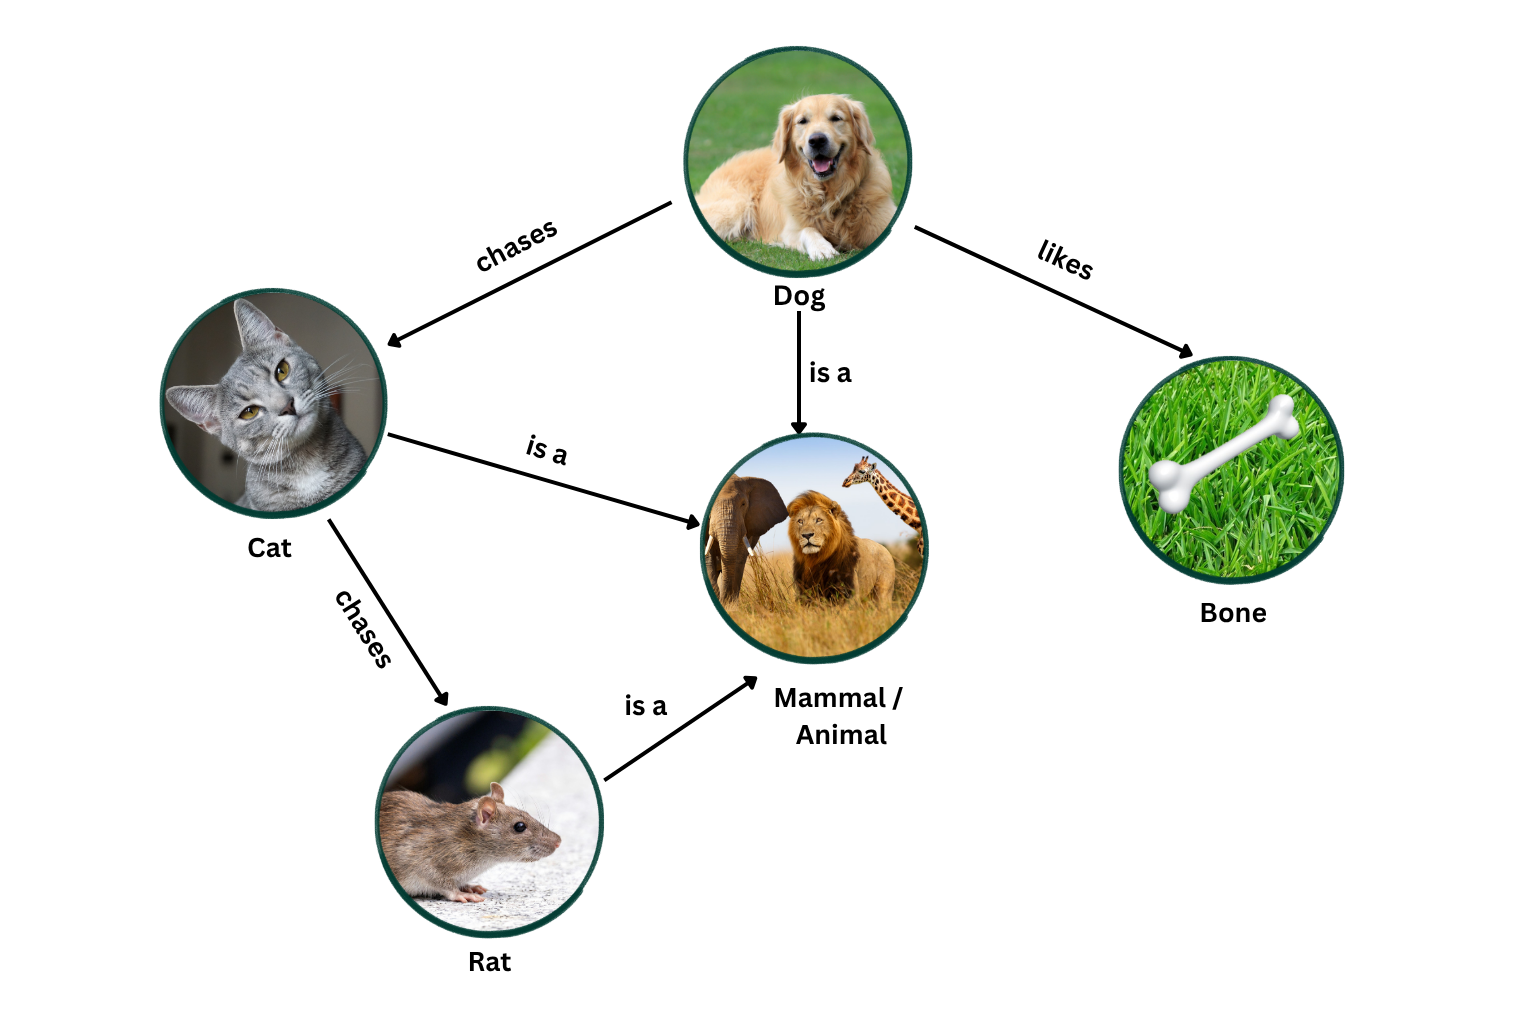
\includegraphics[width=\textwidth]{inc/figures/kg.png}
    \caption{Knowledge Graph Example}
    \label{fig:kgexample}
\end{figure}
For example, Figure~\ref{fig:kgexample} shows a small knowledge graph in
which entities such as a dog, cat, rat, and bone are represented as nodes,
while labelled edges represent relations between them, such as
\textit{chases}, \textit{likes}, and \textit{is a}. The example is deliberately
domain-independent and is intended only to illustrate the basic node--edge
representation of a knowledge graph. In this thesis, the same principle is
applied to clinical guideline concepts, with entities such as drugs,
conditions, guidelines, and clinical targets represented as typed nodes.
The complete clinical schema used in this work is defined later in
Section~\ref{sec:schema}.


\subsection{Graph Data Models}
\label{sec:bg-kg-models}

The internal model chosen for a knowledge graph determines how facts and their
attributes are stored and queried. ~\cite{hogan2021} describe
several models, of which two are relevant to this work: the directed
edge-labelled graph, of which the Resource Description Framework (RDF) is the
best-known instance, and the property graph.

In a directed edge-labelled graph, every fact is a triple that links a subject
node to an object node through a labelled edge, written here as
subject--predicate--object. Any additional detail about an entity, such as a
numerical value or a source reference, has to be expressed as further triples
attached to additional nodes, because an edge in this model carries only its
label~\cite{hogan2021}. RDF follows this model and adds conventions for naming
entities so that graphs published by different parties can be linked together.

A property graph relaxes this restriction. In addition to a type label, each
node and each edge may carry an arbitrary set of key-value
properties~\cite{hogan2021}. A fact such as a recommended dosage or the
guideline a statement came from can therefore be stored directly on the node
or edge it describes, rather than being broken out into separate triples.
~\cite{hartig2014} studies the correspondence between the two models and
shows how graphs can be translated between them, which confirms that the
choice is one of convenience and expressiveness rather than of what can in
principle be represented. The practical consequence is that attributes and
edge-level metadata are more compact to express in a property graph, a point
returned to when the schema of this work is defined in
Chapter~\ref{chap:construction}.

Table~\ref{tab:lpg-rdf} summarises the principal differences between the two
models across the dimensions most relevant to this work.

\begin{table}[htbp]
\centering
\small\setlength{\tabcolsep}{5pt}
\begin{tabular}{p{2.6cm} p{5.2cm} p{5.2cm}}
\hline
\textbf{Feature} & \textbf{Property graph} & \textbf{RDF} \\
\hline
Data structure
  & Typed nodes and edges, each carrying a set of key-value properties
  & Triples: subject -- predicate -- object \\[4pt]
Edge attributes
  & Stored directly on the edge as properties
  & Require intermediate nodes or reification triples \\[4pt]
Schema
  & Optional; the model can be extended at runtime
  & Ontology-driven; defined using RDFS or OWL \\[4pt]
Query language
  & Cypher (used in Neo4j and Memgraph)
  & SPARQL \\[4pt]
Interoperability
  & Local identifiers; suited to single-system deployments
  & Global URIs; supports linked open data across systems \\[4pt]
Primary strength
  & Graph traversal and analytics on highly connected data
  & Semantic reasoning and cross-system data integration \\
\hline
\end{tabular}
\caption{Comparison of property graph and RDF data models.}
\label{tab:lpg-rdf}
\end{table}

\subsection{Knowledge Graphs in the Biomedical Domain}
\label{sec:bg-kg-biomed}

In medicine, knowledge graphs are used to bring together information that is
otherwise scattered across terminologies, structured records, and the research
literature. A common starting point is a controlled vocabulary that assigns a
single identifier to each clinical concept. The Unified Medical Language System integrates many such biomedical
vocabularies into one resource, linking multiple names to a single concept and
providing tools for extracting concepts from text \cite{bodenreider2004}. Ontologies built on standard coding systems, such
as the drug ontology of ~\cite{hanna2013} based on RxNorm, serve a
similar role by providing stable identifiers that let independently produced
data be aligned.

Other work builds biomedical knowledge graphs from clinical text rather than
from vocabularies alone. ~\cite{li2020} construct a medical knowledge
graph from real-world clinical data and apply it to downstream tasks, while
~\cite{harnoune2021} use a BERT-based language model to extract
clinical entities and relations from biomedical documents for graph
construction. These systems generally draw on a single kind of source, most
often electronic health records or the biomedical literature. Knowledge graphs
built specifically from published clinical guidelines, and in particular from
several guidelines issued by different organisations so that their
recommendations can be compared, have received far less attention. That
setting is the focus of this thesis.

\section{Information Extraction}
\label{sec:bg-ie}

Building a knowledge graph from documents requires identifying the entities
mentioned in the text and the relations that hold between them. This section
describes the task and the main families of methods used to perform it.

\subsection{Named Entity Recognition and Relation Extraction}
\label{sec:bg-ie-ner}

The extraction task is usually divided into two parts. Named entity
recognition locates mentions of entities in text and classifies them into
types, such as a drug or a disease. Relation extraction then determines how
those entities are connected, for example that a drug is recommended for a
condition~\cite{nasar2021}. Together the two tasks turn unstructured text into
the typed nodes and edges that a knowledge graph is composed of. Both are
long-standing problems in natural language processing, and ~\cite{nasar2021} survey the range of methods that have been applied to
them.

\subsection{Rule-Based and Learning-Based Methods}
\label{sec:bg-ie-methods}

Approaches to information extraction fall broadly into rule-based and
learning-based methods. Rule-based extraction relies on hand-written patterns,
such as regular expressions or dictionaries of known terms, that match the way
information is stated in a particular kind of text.\cite{chiticariu2013} observe that rule-based information extraction dominates
the commercial world even though it is widely regarded as a dead end in
academic research, and note that practitioners value rule-based systems for
their interpretability. Rules are also a natural fit for text where the
relevant facts follow a predictable form, such as a numerical threshold or a
graded recommendation, because a small number of patterns can cover most of the
cases.
Learning-based extraction instead trains a model on annotated examples. Deep
learning models, in particular hybrid and joint models for named entity
recognition and relation extraction, now represent the state of the art
\cite{nasar2021}, and pre-trained language models fine-tuned for relation
extraction have outperformed earlier systems on clinical shared tasks
\cite{wei2020}. In the clinical domain, \cite{harnoune2021} use a BERT-based
model with a conditional random field layer to extract entities and relations
from clinical notes. Shared tasks such as the i2b2 and n2c2 challenges evaluated
systems for extracting concepts, assertions, medications, adverse drug events
and the relations between them from clinical narratives
\cite{uzuner2011,henry2020}. Learning-based methods depend on annotated
training data, which is scarce for many domains, and understanding the
decisions made inside deep architectures remains difficult \cite{nasar2021}.

\subsection{Hybrid Approaches}
\label{sec:bg-ie-hybrid}

Because the two families have complementary strengths, some systems combine
them.~\cite{chiticariu2013} argue for rule-based components
where precision and control matter, and hybrid designs that pair hand-written
rules with machine learning have been used in text-processing tasks to obtain
the reliability of rules together with the coverage of learned
models~\cite{villena2011}. Large language models have more recently been applied
to extraction as a further alternative, discussed in the next section. The
extraction stage of this work draws on a combination of rule-based and
learning-based methods, assigning each to the part of the task for which it is
better suited; the details are given in Chapter~\ref{chap:construction}.

\section{Grounding Language Model Output}
\label{sec:bg-grounding}

Large language models can produce fluent and plausible text, but they are
prone to generating statements that are not supported by any real source. This
section describes the problem and the techniques used to constrain model output
to reliable information.

\subsection{Hallucination in Language Models}
\label{sec:bg-grounding-hallucination}

The generation of unsupported or incorrect content by a language model is known
as hallucination. ~\cite{huang2025} distinguish two forms.
Factuality hallucination is when the output contradicts verifiable facts about
the world. Faithfulness hallucination is when the output departs from the input
or context the model was given, even where it is not wrong in a general sense.
They attribute this behaviour in part to the fact that the models are trained
to produce coherent and probable text, which does not by itself guarantee that
the text is factually correct. In a clinical setting this is a serious concern,
because a confidently worded but incorrect statement about a treatment or a
threshold could mislead a reader who is not in a position to check it.

\subsection{Retrieval-Augmented Generation}
\label{sec:bg-grounding-rag}

One established way to reduce hallucination is to ground generation in an
external source of knowledge rather than relying on what the model has stored
in its parameters. ~\cite{lewis2021} introduce retrieval-augmented
generation, which combines the parametric memory held in the model's weights
with a non-parametric memory in the form of an external document store. At
generation time the system retrieves relevant passages and conditions the
output on them, so that the generated text is tied to retrieved evidence. The
authors report that this grounding improves factual accuracy and provides a way
to trace an output back to the source it was drawn from. The same principle
underlies a range of later systems that constrain a language model to
information supplied at generation time rather than allowing it to draw freely
on its parameters.

\subsection{Schema-Constrained Generation}
\label{sec:bg-grounding-schema}

Providing a model with an explicit, structured input is a strong form of this
grounding. ~\cite{caufield2024} show that prompting a language
model with a defined schema constrains its output to the structure and content
requested, which is useful when the goal is to extract or generate information
that must conform to a fixed set of types. The question generation stage of
this work follows the same idea: rather than asking a language model to produce
clinical questions from its own knowledge, it supplies a single fact drawn from
the knowledge graph and constrains the model to that fact. Grounding of this
kind has been studied mainly for retrieval from text corpora; grounding
generation in a structured knowledge graph built from clinical guidelines, so
that every generated question is tied to a specific guideline statement, is
less commonly addressed. How this is done, and how the output is checked
against the supplied fact, is described in Chapter~\ref{chap:construction}.

\section{Automatic Question Generation}
\label{sec:bg-qg}

Generating questions automatically from a source of knowledge is an active
area of research in natural language processing, motivated by applications
in education, information retrieval, and dialogue systems. This section
reviews the main approaches and the educational framework used to describe
what different kinds of questions demand from a learner.

\subsection{Approaches to Question Generation}
\label{sec:bg-qg-approaches}

Early question generation systems used rule-based templates that transformed
a declarative statement into an interrogative form by pattern substitution.
These systems produce grammatical output reliably but are limited to the
question types for which templates have been written and lack the flexibility
to vary phrasing. Neural approaches have since been developed that learn to
generate questions directly from text or from structured knowledge sources.
~\cite{guo2024} survey the range of neural methods applied to
question generation, covering inputs including free text, knowledge bases, and
images. They report that knowledge-base question generation, where the input
is a set of structured facts rather than a passage of text, poses particular
challenges because the model must convert a formal relation triple into a
natural language question that accurately reflects both the entities and the
direction of the relationship.

Large language models have also been applied to knowledge-base question
generation, for example in few-shot settings where labeled data is scarce.
\cite{liang2023} propose KQG-CoT, which retrieves supportive logical forms
from an unlabeled pool and prompts an LLM to build a complex question as a
chain of sub-questions. A variant, KQG-CoT+, orders the demonstrations by
complexity and improves on the previous few-shot state of the art on
PathQuestions. \cite{guo2024} note in their survey that the central challenge
for LLM-based KBQG is designing prompts that steer the model toward the
intended question.

Question generation from clinical knowledge has received some specific
attention. ~\cite{nyameino2020} describe a system that
generates questions automatically from a clinical guideline, using the
guideline structure to drive the question type and content. The questions
produced cover individual recommendations taken from the guideline, rather
than comparing recommendations across several guidelines from different
organisations.

\subsection{Multiple-Choice Question Generation}
\label{sec:bg-qg-mcq}

Multiple-choice questions require, in addition to a correct answer, a set of
plausible but incorrect options, known as distractors, that a learner who does
not know the material might plausibly select. \cite{gao2019} address
distractor generation for reading comprehension questions, using a
hierarchical encoder-decoder with attention to generate longer, semantically
rich distractors from the article, the question, and the correct option. In a
clinical context, plausible distractors are typically other drugs or other
thresholds from the same domain, which makes a knowledge graph a natural
resource for distractor selection because it contains the set of all relevant
alternatives as named nodes.

\subsection{Educational Taxonomies and Difficulty}
\label{sec:bg-qg-bloom}

The cognitive demand of a question is typically described using a taxonomy of
learning objectives. ~\cite{anderson2001} revised the
original taxonomy proposed by Bloom to organise cognitive processes along six
levels: remember, understand, apply, analyse, evaluate, and create. The
revision shifted the original noun-based category names to verbs in order to
emphasise that these are active processes, and it moved the creation category
to the highest level to reflect that generating new constructs requires more
than evaluation alone. The lower levels, remember and understand, correspond
broadly to the ability to recall and interpret factual information, while
apply, analyse, and evaluate require the learner to use and reason with that
information in increasingly open-ended ways.

In question design, this hierarchy is used to classify the cognitive level a
question targets. A question that asks for the value of a specific diagnostic
threshold requires recall; a question that presents a clinical scenario and
asks which management option is appropriate requires application. Generating
questions at a range of levels produces a catalogue that tests different
depths of understanding rather than a single level of recall. This work
assigns a difficulty level to each generated question based on the relation
type that the question was built from, using the Bloom hierarchy as a guide,
as described in Chapter~\ref{chap:construction}.

Table~\ref{tab:bloom} shows the six cognitive levels of the revised taxonomy
together with the kind of question activity associated with each, based on
~\cite{anderson2001}.

\begin{table}[htbp]
\centering
\small\setlength{\tabcolsep}{5pt}
\begin{tabular}{p{0.5cm} p{2.2cm} p{7.8cm}}
\hline
& \textbf{Process} & \textbf{Associated question activity} \\
\hline
& Remember    & Recall or recognise a specific fact, term, or value \\[3pt]
& Understand  & Explain or restate a concept in one's own words \\[3pt]
& Apply       & Use a known fact or procedure to answer a new question or solve a case \\[3pt]
& Analyse     & Break a scenario into parts and identify how they relate \\[3pt]
& Evaluate    & Judge or justify a clinical decision against given criteria \\[3pt]
& Create      & Design, compose, or propose something novel from existing knowledge \\
\hline
\end{tabular}
\caption{Cognitive levels in the revised Bloom taxonomy.}
\label{tab:bloom}
\end{table}

\section{Clinical Practice Guidelines}
\label{sec:bg-guidelines}

Clinical practice guidelines are systematically developed statements that
summarise the available clinical evidence on a topic and translate it into
recommendations for practice \cite{nyameino2020}. Their purpose is to improve
the quality of care and reduce unjustified variation in practice
\cite{peleg2013}. Many guidelines grade the quality of the underlying evidence
and the strength of each recommendation, most commonly using the GRADE system
\cite{guyatt2011}. In the diabetes domain
the organisations whose guidelines are used in this work each produce such
statements independently, drawing on their own review processes and addressing
their respective healthcare systems and populations.

\subsection{Evidence Grading and Recommendation Structure}
\label{sec:bg-guidelines-grade}

Many guideline producers use a structured grading system to convey the
strength of the underlying evidence and the force of each recommendation.
One widely used framework is the Grading of Recommendations Assessment,
Development and Evaluation system, known as GRADE, which rates the quality of
evidence and grades recommendations as strong or weak according to the quality
of the evidence and the balance of desirable and undesirable consequences
\cite{guyatt2011}.
Under GRADE, evidence quality is rated from high to very low depending on study
design, consistency of findings, and precision, and recommendations are then
graded as strong or conditional based on both the quality of evidence and the
balance of benefits against harms. The GRADE system produces recommendations
that carry explicit markers of how much confidence a clinician should place in
them, which makes the recommendation label a meaningful structured field rather
than a narrative qualifier.

In practice, the issuing organisations whose guidelines this work uses do not
all follow exactly the same grading system. The ADA uses lettered grades
(A through E), NICE uses strength ratings tied to the quality of its evidence
review, and Diabetes Canada uses a graded classification from A to D.
Regardless of the specific notation, all four organisations distinguish
stronger from weaker recommendations in a structured way, and this structure
is part of what the ingestion stage of this work captures.

\subsection{Computer-Interpretable Guidelines}
\label{sec:bg-guidelines-cig}

Making guideline content available to computational systems requires moving
beyond the PDF and word-processed documents in which guidelines are typically
published. ~\cite{peleg2013} provides a methodological review of
computer-interpretable guidelines, a line of research that formalises clinical
guidelines as executable or queryable representations. The review covers
modelling languages and acquisition methodologies developed over roughly two
decades, and it identifies as a central challenge the gap between the natural
language in which clinical guidelines are written and the formal structures
that a computer can evaluate. The representations covered by Peleg range
from flow-chart-based models to logic-based formalisms, and the work reports
that translating a narrative guideline into any of these forms remains
time-consuming and requires significant expert input.

Approaches that use artificial intelligence to assist or automate this
translation have attracted increasing interest. Large language models can
extract structured information from text with little or no task-specific
training data \cite{xu2024, caufield2024}, which suggests they could also help
turn narrative guidelines into structured form. This thesis takes a related
but distinct approach: rather than formalising a guideline into a decision
model, it extracts the entities and relations that a guideline states into a
property graph, so that the content of several guidelines can be queried and
compared in a common structure. The difference is in purpose:
computer-interpretable guidelines aim at decision support and care pathway
execution, while the knowledge graph constructed in this work aims at
information integration and study question generation across multiple
guideline sources. Question generation in this setting has so far mainly
supported guideline development: \cite{sousa-pinto2024} prompted LLMs to
propose guideline questions and found that some were not previously raised by
the guideline panel.

\section{Related Work}
\label{sec:bg-related}

This section discusses the work most closely related to this thesis and sets
out how the present work differs from it. The preceding sections have
reviewed individual technical components in isolation; here the focus is on
systems that combine several of those components toward a goal comparable to
the one pursued here.

\paragraph{Knowledge Graph Construction from Clinical Text}
\label{sec:bg-related-kg}

Several systems construct biomedical knowledge graphs from clinical text
using extraction pipelines that combine named entity recognition with relation
extraction.~\cite{li2020} build a medical knowledge graph from
real-world clinical data records, and ~\cite{harnoune2021}
extract clinical knowledge from biomedical documents using a BERT-based model.
Both systems work on a single document collection of one type, either
electronic health records or biomedical literature, and neither addresses the
problem of combining content from multiple separately produced guidelines that
each use different structural conventions and different units of measurement.
The present work is distinguished by its explicit treatment of structural
heterogeneity across sources and its normalisation of measurement units so
that numerical thresholds from different guidelines can be directly compared.
\paragraph{Question Generation from Clinical Knowledge}
\label{sec:bg-related-qg}

Question generation from structured knowledge has developed as a distinct
research direction as knowledge graphs have grown richer and more queryable.
~\cite{bi2020} generate questions from knowledge bases using
explicit type constraints and grammar guidance, showing that the structural
properties of a knowledge source can be used to control the factual content
and form of generated questions. ~\cite{guo2024} survey neural question generation across knowledge bases, text, and images,
organize the literature into structured, unstructured, and hybrid NQG, and
note that knowledge-base question generation benefits from models that
preserve graph structure and mark the roles of heads, relations, and tails
rather than treating a subgraph as a flat sequence of triples. Prompting a language model with structured input rather than asking it to
generate freely is a common design in knowledge-base question generation
\cite{liang2023}, and constraining output to supplied content is also used to
reduce unsupported statements \cite{huang2025}.

In the clinical domain specifically, ~\cite{nyameino2020}
describe a system that generates questions automatically from a single
clinical guideline for use in a gamified training setting. Their work is the
closest antecedent to the question generation component of this thesis and
establishes that guideline content can be turned into assessment questions
automatically.

This thesis extends that line of work in two ways. First, the input is a
knowledge graph built from four guidelines rather than a single source
document, which makes cross-guideline questions possible. Second, each
question is grounded to a specific graph edge selected before the language
model is called, and every generated question is validated against that
anchor. Questions derived from \textsc{equivalent\_to} edges, which connect
nodes from different organisations that assert the same numerical threshold,
require knowledge of how two guidelines compare and are not possible from a
single-guideline source.

\paragraph{AI-Assisted Guideline Processing}
\label{sec:bg-related-ai-guidelines}

\cite{sousa-pinto2024} examine how large language models can support the
development of guideline questions, using the ARIA 2024 guidelines as a single
case study, and \cite{peleg2013} reviews the broader effort to produce
computer-interpretable representations of individual guidelines for use in
decision support. Neither addresses the representation of several guidelines
together. The goal of this thesis is different: it is not to execute guidelines
as decision logic but to represent the content of several guidelines in a
common structure that can answer questions about how those guidelines agree,
differ, and complement one another.
